\chapter{Problemanalyse}

Det første skridt mod et program er ofte et mockup. Et mockup visualiserer en idé, og får en brainstorm til at være mere konkret. Ud fra dette bliver der arbejdet med hvert enkle element i mockup'en, hvilket ofte gør, at hvert element bliver en klasse i en kode. Ud fra mockup'en er det også lettere at se hvilke klasser skal være forbundet til hinanden, og derefter også hvor data skal placeres (hvis data skal være med).

\section{Beskrivelse}

Vi har valgt at bruge et program (ud af mange) der hedder Balsamiq Mockups.
Det står i problemformuleringen, at Bookie ikke skal være indviklet, hvilket bliver reducéret ti, at Bookie kun skal kunne det mest basale, som et reservationssystem kræver. Data er en nødvendighed, men der er forskellige måder at repræsentere den på.

Ud fra vores mockup, repræsenterer vi data på den måde, at der først bliver valgt en film (\ref{mockup: balsamiq-showtimes}), hvorefter man kommer ind på et vindue, hvor der er muligt at se hvilke dage og tidspunkter den valgte film bliver vist (\ref{mockup: balsamiq-showtimes1}). Inde på næste vindue bliver det så muligt at reservere pladser (\ref{mockup: balsamiq-auditorium}), hvilke så ender inde på \textit{Reservationer} (\ref{mockup: balsamiq-reservation}).

I forhold til vores mockup, er der på startsiden (\ref{mockup: balsamiq-showtimes}) lavet en liste som repræsenterer filmene som data. Til hver film er der en tabel (\ref{mockup: balsamiq-showtimes1}), hvor rækkerne beskriver tidspunkter på dagen, og kolonnerne dagene i ugen. Til hver forestilling er der en sal (\ref{mockup: balsamiq-auditorium}), hvor sæderne er delt op i et gitter, og hvor hvert sæde repræsenterer en billet. Hvilket inkluderer i, at en billet er forbundet med et tidspunkt og en sal, som er forbundet til en film. Dog har \textit{Reservationer} også en liste, men denne liste indeholder billetter. Det vil sige, at billetterne også er forbundet til \textit{Reservationer}, men ikke omvendt.

Inde på \textit{Reservationer} er der også muligt at søge efter en bestemt reservation ved at skrive et telefonnummer ind på \textit{søg}-feltet. Dette felt vil så filtrere numrene i tabellen.

Idéen fungerer fint, men JavaFX har ikke samarbejdet på et optimalt plan, hvilket har fået den endelige brugergrænseflade til at blive lidt anderledes, den har en lidt anden måde at repræsentere data på. Som det også kan ses i \textit{Brugervejledning og eksempel}, så er alle forestillinger i samme tabel, med salene til højre for tabellen. Igen er data fra reservationerne repræsenteret i et gitter. \textit{Reservationer} i Bookie minder meget om mockup'en. 


\subsection{Mockups}

\begin{figure}[h]
  \centering
  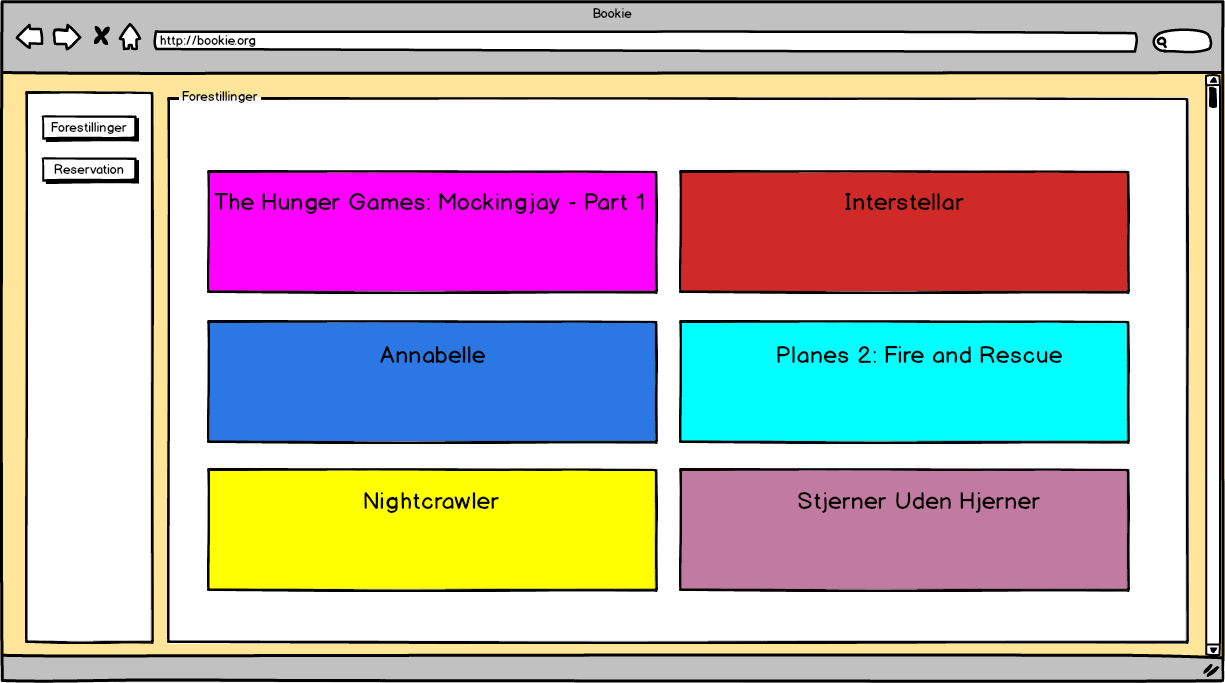
\includegraphics[width=\textwidth]{balsamiq-showtimes.png}
  \caption{Mockup - Bookie startside}
  \label{mockup: balsamiq-showtimes}
\end{figure}

\begin{figure}[h]
  \centering
  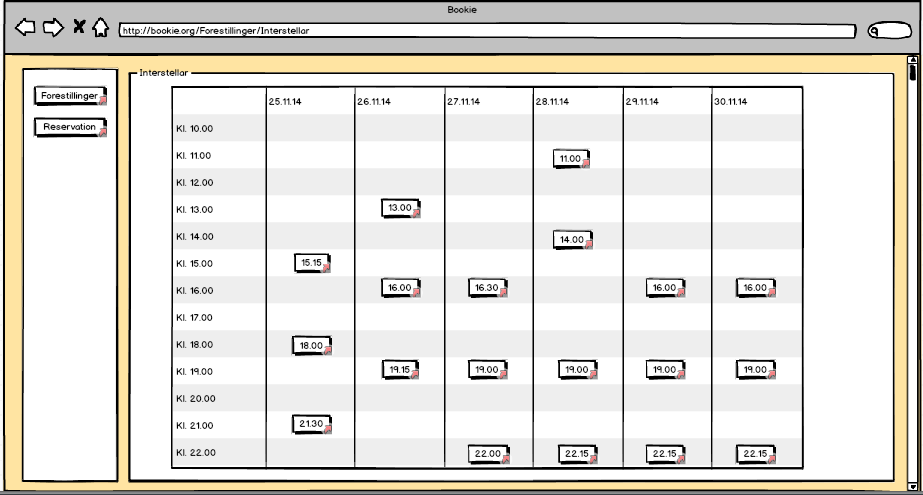
\includegraphics[width=\textwidth]{balsamiq-showtimes1.png}
  \caption{Mockup - tidspunkter}
  \label{mockup: balsamiq-showtimes1}
\end{figure}

\begin{figure}[h]
  \centering
  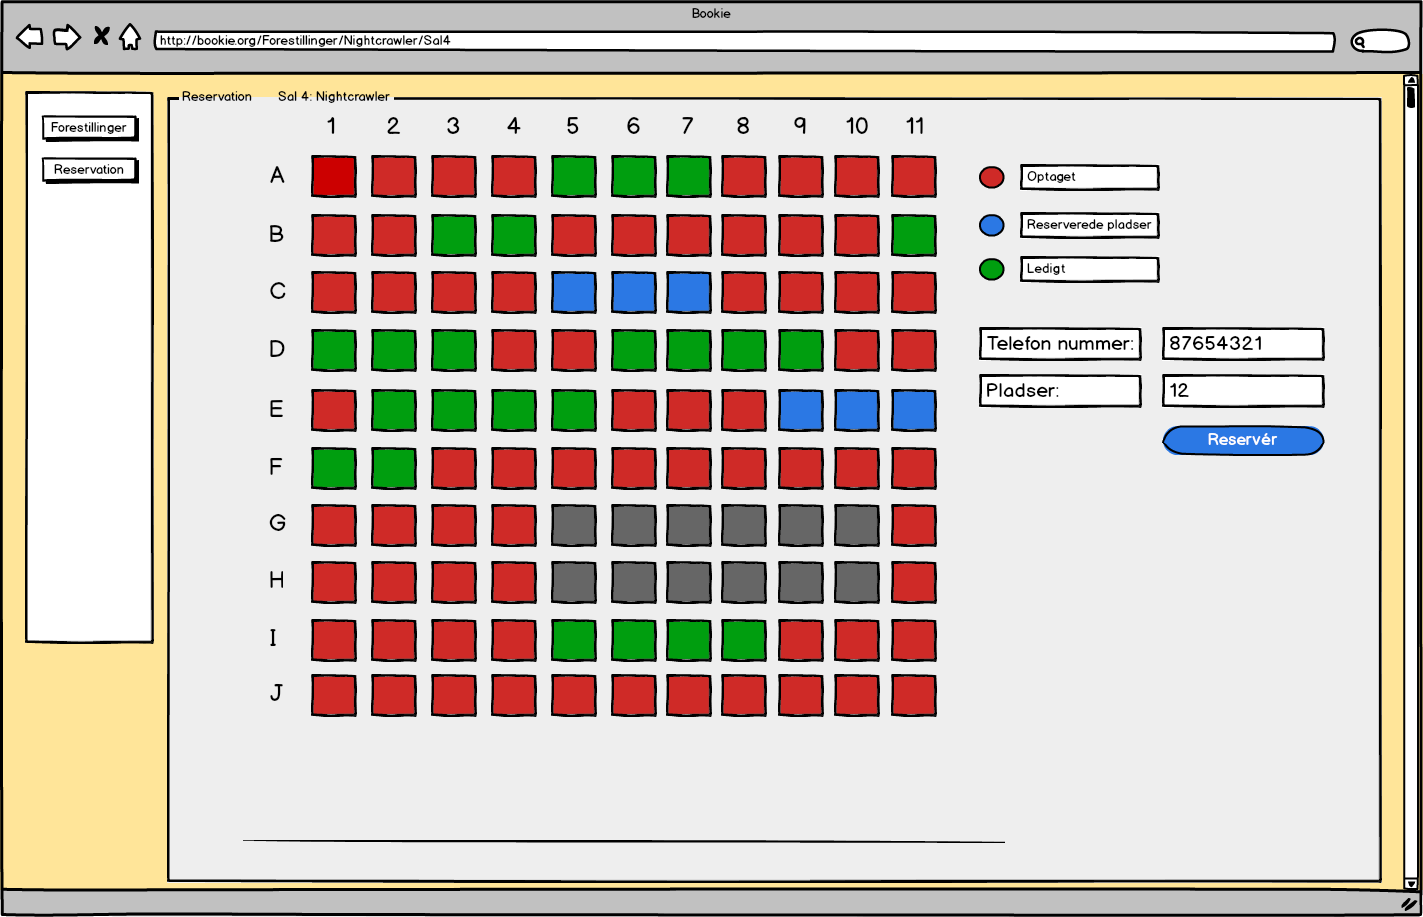
\includegraphics[width=\textwidth]{balsamiq-auditorium.png}
  \caption{Mockup - Eksempel af en sal}
  \label{mockup: balsamiq-auditorium}
\end{figure}

\begin{figure}[h]
  \centering
  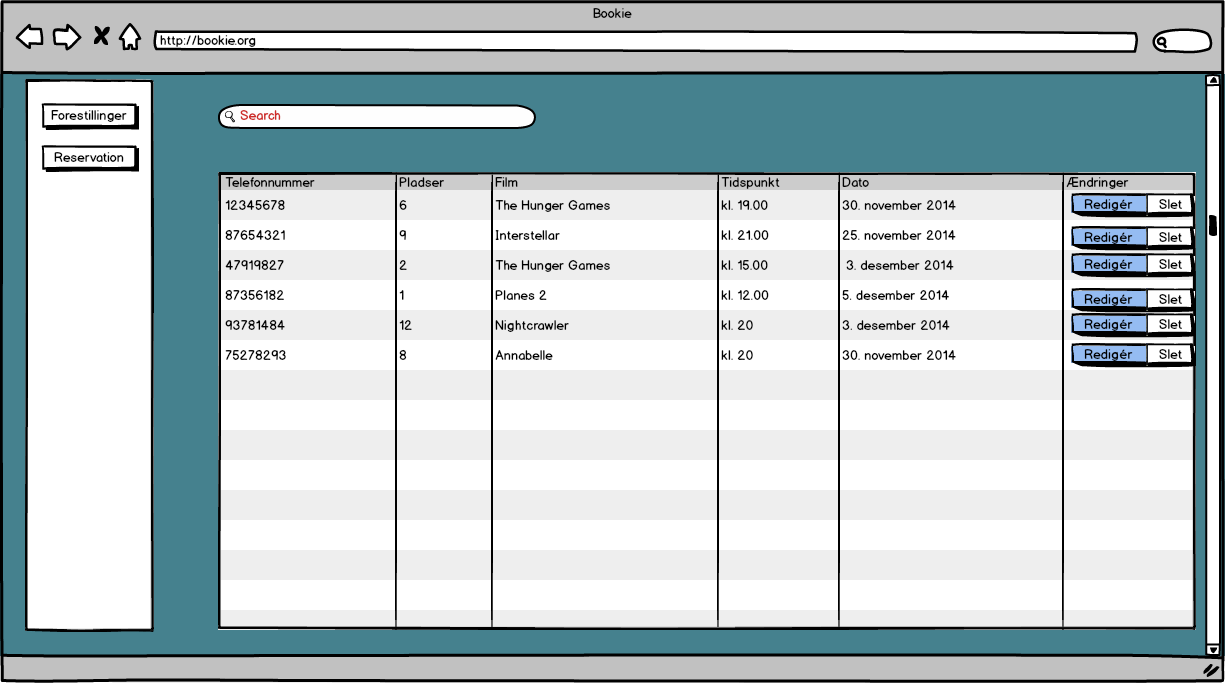
\includegraphics[width=\textwidth]{balsamiq-reservation.png}
  \caption{Mockup - Reservationer}
  \label{mockup: balsamiq-reservation}
\end{figure}

\section{Diskussion}

\section{Databasedesign}

Bookies databasedesign (\ref{class-diagram: bookie-models}) viser os klassernes forhold til hinanden. Databasen er opbygget på den måde, at hver klasse i \textit{Model} er en række, og hvert felt i klasserne er en kolonne. Der er tilføjet en forklaring for hver enkelte klasse.

\begin{figure}[h]
  \centering
  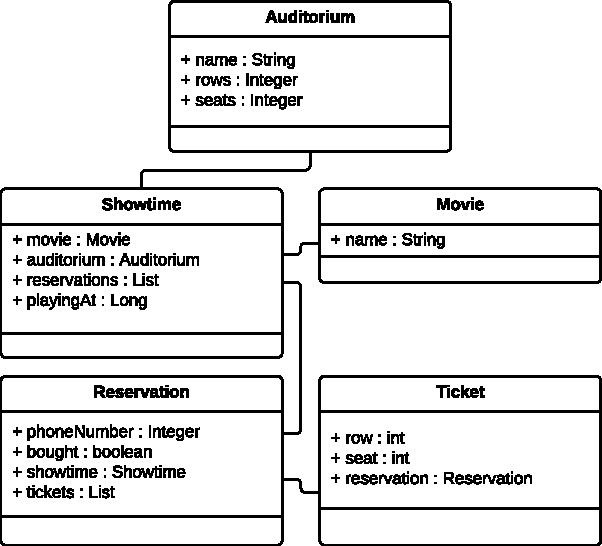
\includegraphics[width=0.6\textwidth]{bookie-models.pdf}
  \caption{Bookies databasedesign}
  \label{class-diagram: bookie-models}
\end{figure}

\subsection{Auditorium}

En sal kan godt eksistere unden nogle af de andre felter, men ikke omvendt.\textit{Auditorium} har tre felter, hvilket inkluderer at rækken har tre kolonner.
\begin{itemize}

  \item \textit{name} er af typen \textit{String} kan kun have strenge som data i kolonnen, hvilket fortæller os navnet på selve salen.
  \item \textit{rows} er sædernes rækker og har typen \textit{Integer}. På grund af at koden er skrevet til ikke at kunne returnere \textit{Null}, men hvis typen havde været den primitive type \textit{int}, så ville det være en mulighed, at biografen ikke havde nogle rækker og det vil sige: ingen rækker. I koden er der automatisk taget forbehold for at ingen kolonner kan være \textit{Null}.
  \item \textit{seats} har også typen \textit{Integer} af samme grund. Der kan ikke være ingen sæder i salen.

\end{itemize}

\subsection{Movie}

\begin{itemize}

  \item \textit{Movie} har kun ét felt med navnet \textit{name} og har typen \textit{String}. Den er kun forbundet til \textit{Showtime}, da ingen af de andre klasser har en direkte forbindelse til \textit{Movie}.

\end{itemize}

\subsection{Reservation}

Denne klasse har fire felte: \textit{phoneNumber, bought, showtime} og \textit{tickets}.

\begin{itemize}
  \item \textit{phoneNumber} er af typen \textit{Integer}, da der må være et telefonnummer forbundet til en reservation, hvis typen havde været \textit{int}, så ville det være muligt med \textit{0} telefonnumre, hvilket det ikke skal.
  \item \textit{bought} er af typen \textit{boolean}, hvilket fortæller os, om reservationen er betalt for, eller ikke. 
  \item \textit{showtime} med typen \textit{Showtime} viser os, at \textit{Reservation} har et forhold til klassen \textit{Showtime}. Forklaring følger i sektionen om \textit{Showtime} .
  \item \textit{tickets} har typen \textit{List}, da en reservation kan have flere billetter. Dette er en \textit{One-to-many}-forhold (\cite{https://learnit.itu.dk/pluginfile.php/114939/mod_resource/content/0/GRPRO-14.pdf}).

\end{itemize}

\subsection{Showtime}

\begin{itemize}
  \item \textit{movie} har typen \textit{Movie}, da en forestilling kan ikke eksistere uden en film, men en film kan godt eksistere uden en forestilling (Den behøver ikke at blive vist på noget tidspunkt). Hvilket betyder, at den har et forhold til klassen \textit{Movie}.
  \item \textit{auditorium} har typen \textit{Auditorium}, som viser os, at en Forestilling bliver nødt til at have en sal for at blive vist. 
  \item \textit{reservatrions} har typen \textit{List}, da en forestilling godt kan have flere reservationer. Dette bliver igen kaldt et \textit{One-to-many}-forhold.
  \item \textit{playingAt} fortæller os hvad tidspunkt forestillingen er. \textit{playingAt} har til gengæld typen \textit{Long}. 
\end{itemize}

\subsection{Ticket}

\begin{itemize}
  \item \textit{row} har typen \textit{Integer}, af samme grund som i \textit{Auditorium}.
  \item \textit{seat} har også typen \textit{Integer}, og igen af samme grund som tidligere. I forhold til \textit{Auditorium} ville det være muligt at have den primitive type \textit{int} i dette felt, men så ville alle kolonnerne i gitteret starte med tallet \textit{0} , hvilket vi har valgt, at det ikke skal gøre, men starte med \textit{1} i stedet.
  \item \textit{reservation} har typen \textit{Reservation}, og viser at der er et forhold til \textit{Reservation} klassen.
\end{itemize}



